% !TeX program = xelatex
\documentclass[aspectratio=169,12pt,fontset=none,usepdftitle=false]{ctexbeamer}
\usepackage{fontspec,amsmath,booktabs,array,tabularx,graphicx,etoolbox}
\usepackage{tikz}
\usetikzlibrary{arrows.meta,positioning,calc}
% sonnyhcl/beamerthemefdu (Apache-2.0); original kept in vendor-fdu/.
\makeatletter
\def\input@path{{vendor-fdu/}}
\makeatother
\usetheme{fdu}
\usefonttheme{professionalfonts}
\setsansfont{Arial}
\setmainfont{Arial}
\setCJKmainfont{Microsoft YaHei}[BoldFont=Microsoft YaHei Bold]
\setCJKsansfont{Microsoft YaHei}[BoldFont=Microsoft YaHei Bold]
\setCJKmonofont{Microsoft YaHei}
\definecolor{Navy}{HTML}{173955}
\definecolor{Blue}{HTML}{1C61A0}
\definecolor{Teal}{HTML}{137E79}
\definecolor{Ochre}{HTML}{A47422}
\definecolor{Ink}{HTML}{253544}
\definecolor{Muted}{HTML}{697987}
\definecolor{Line}{HTML}{D5DEE5}
\definecolor{Pale}{HTML}{F2F5F8}
\definecolor{PaleBlue}{HTML}{ECF2F9}
\definecolor{PaleTeal}{HTML}{EAF5F2}
\definecolor{PaleGold}{HTML}{F8F2E6}
\setbeamercolor{normal text}{fg=Ink,bg=white}
\setbeamercolor{structure}{fg=Blue}
\setbeamercolor{frametitle}{fg=Navy,bg=white}
\setbeamercolor{title}{fg=Navy,bg=white}
\setbeamercolor{subtitle}{fg=Ink,bg=white}
\setbeamerfont{frametitle}{size=\fontsize{21}{26}\selectfont,series=\bfseries}
\setbeamersize{text margin left=8mm,text margin right=8mm}
\setbeamertemplate{navigation symbols}{}
\setbeamertemplate{background canvas}{}
\setbeamertemplate{itemize item}{\raisebox{.2ex}{\scriptsize\textcolor{Blue}{\textbullet}}}
\setlength{\parskip}{.12em}
\renewcommand{\arraystretch}{1.18}
\newcommand{\NavItem}[2]{\ifnum\value{section}=#1\textcolor{Blue}{\bfseries #2}\else\textcolor{Muted}{#2}\fi}
\setbeamertemplate{headline}{%
  \vspace{2mm}\hspace{8mm}%
  {\fontsize{9}{11}\selectfont\NavItem{1}{选题与数据}\hspace{8mm}\NavItem{2}{当前进展}\hspace{8mm}\NavItem{3}{后续计划}}\par\vspace{1mm}%
}
\setbeamertemplate{frametitle}{%
  \vspace{-1mm}\usebeamerfont{frametitle}\insertframetitle\par\vspace{1.2mm}%
  {\color{Line}\hrule height .6pt}%
}
\setbeamertemplate{footline}{%
  \hspace{8mm}\begin{minipage}{\dimexpr\paperwidth-16mm\relax}%
  {\color{Line}\hrule height .35pt}\vspace{1mm}%
  {\fontsize{7.5}{9}\selectfont\color{Muted}FinGraph\hfill 知识图谱课程 · 期中汇报\hfill\insertframenumber\,/\,\inserttotalframenumber}\par\vspace{1mm}%
  \end{minipage}%
}
\newcommand{\Intro}[1]{{\fontsize{12.2}{16}\selectfont #1}\par\vspace{2mm}}
\newcommand{\Head}[1]{\par{\color{Blue}\bfseries #1}\par\vspace{.5mm}}
\newcommand{\Caption}[1]{\par{\fontsize{9.5}{12}\selectfont\color{Muted}#1}\par}
\newcommand{\Gap}{\par\vspace{2mm}}
\tikzset{entity/.style={draw=Line,fill=white,rounded corners=1mm,align=center,
  minimum height=.8cm,text width=2.2cm,inner sep=1.4mm,font=\fontsize{11.5}{14}\selectfont},
  rel/.style={-{Stealth[length=1.8mm]},draw=Blue,line width=.9pt},
  edge label/.style={font=\fontsize{10}{12}\selectfont,text=Muted,fill=white,inner sep=.7mm}}
\graphicspath{{resources/}{generated/}}
% Generated from actual delivered data; do not hand-edit.
\newcommand{\GraphNodeCount}{59}
\newcommand{\GraphEdgeCount}{85}
\newcommand{\SourceCount}{41}
\newcommand{\EventCount}{10}
\newcommand{\StockCount}{8}
\newcommand{\ValidationCount}{24}
\newcommand{\ApiCheckCount}{20}
\newcommand{\LiveModelName}{DeepSeek V4.1 Flash}
\newcommand{\LiveElapsedSeconds}{14.5}
\newcommand{\GLMAnchorDate}{2026-02-13}
\newcommand{\CoverageStart}{2025-01-20}
\newcommand{\CoverageEnd}{2026-02-14}
\newcommand{\ModelCount}{4}
\newcommand{\MarketCount}{2}
\newcommand{\MarketSeriesCount}{10}
\newcommand{\MarketRowCount}{2448}
\newcommand{\GLMCurrentStockCount}{2}
\newcommand{\GLMHistoricalStockCount}{1}
\newcommand{\GLMPathCount}{2}
\newcommand{\GLMBenchmarkFive}{-1.64\%}
\newcommand{\GLMExcessFive}{+57.85}
\newcommand{\GLMPostUpdateStockCount}{3}
\newcommand{\UpdateNodeCount}{1}
\newcommand{\UpdateEdgeCount}{3}
\newcommand{\GLMReturnOne}{+20.65\%}
\newcommand{\GLMReturnThree}{+80.35\%}
\newcommand{\GLMReturnFive}{+56.22\%}

% Derived from the actual graph, market cache and audit output; do not hand-edit.
% Regenerate with: python docs/presentation/derive_research.py
\newcommand{\EntityTypeCount}{6}
\newcommand{\RelationTypeCount}{8}
\newcommand{\TotalPathCount}{8}
\newcommand{\MaxHops}{4}
\newcommand{\GLMCurrentStocks}{2}
\newcommand{\GLMHistoricalStocks}{1}
\newcommand{\LiveNodeCount}{59}
\newcommand{\LiveEdgeCount}{85}
\newcommand{\LiveSourceCount}{41}
\newcommand{\LiveEventCount}{10}
\newcommand{\LiveStockCount}{8}
\newcommand{\LiveModelCount}{9}
\newcommand{\GLMCurrentPaths}{2}
\newcommand{\DeepSeekStartStocks}{0}
\newcommand{\DeepSeekFebThreeStocks}{2}
\newcommand{\DeepSeekFebFiveStocks}{4}
\newcommand{\DeepSeekCurrentStocks}{4}
\newcommand{\DeepSeekFebThreeSymbols}{00700.HK、09888.HK}
\newcommand{\DeepSeekFebFiveSymbols}{00700.HK、00728.HK、09888.HK、688041.SH}
\newcommand{\DeepSeekCurrentSymbols}{00700.HK、00728.HK、09888.HK、688041.SH}
\newcommand{\QwenEventStocks}{2}
\newcommand{\QwenCurrentStocks}{3}
\newcommand{\QwenEventSymbols}{09988.HK、688041.SH}
\newcommand{\QwenCurrentSymbols}{09988.HK、688041.SH、688795.SH}
\newcommand{\GLMHistoricalPaths}{1}
\newcommand{\GLMCurrentRoles}{2}
\newcommand{\GLMHistoricalRoles}{1}
\newcommand{\GLMAfterUpdatePaths}{3}
\newcommand{\MiniMaxCurrentPaths}{3}
\newcommand{\MiniMaxHistoricalPaths}{1}
\newcommand{\MiniMaxExcludedCount}{2}
\newcommand{\AdaptCurrentPaths}{3}
\newcommand{\AdaptHistoricalPaths}{2}
\newcommand{\GLMAfterUpdateStocks}{3}
\newcommand{\GLMCurrentSymbols}{02513.HK、09988.HK}
\newcommand{\GLMHistoricalSymbols}{02513.HK}
\newcommand{\GLMAfterUpdateSymbols}{02513.HK、09988.HK、688795.SH}
\newcommand{\GLMDirectCount}{1}
\newcommand{\GLMDistributionCount}{1}
\newcommand{\MiniMaxCurrentStocks}{3}
\newcommand{\MiniMaxHistoricalStocks}{1}
\newcommand{\MiniMaxCurrentSymbols}{00100.HK、09988.HK、688795.SH}
\newcommand{\MiniMaxHistoricalSymbols}{00100.HK}
\newcommand{\AdaptCurrentStocks}{3}
\newcommand{\AdaptHistoricalStocks}{2}
\newcommand{\AdaptCurrentSymbols}{00100.HK、09988.HK、688795.SH}
\newcommand{\AdaptHistoricalSymbols}{00100.HK、688795.SH}
\newcommand{\UpdateNewNodes}{1}
\newcommand{\UpdateNewEdges}{3}
\newcommand{\UpdateNewStocks}{1}
\newcommand{\UpdateNewStockSymbols}{688795.SH}
\newcommand{\GLMReleaseDate}{2026-02-12}
\newcommand{\MiniMaxReleaseDate}{2026-02-12}
\newcommand{\AdaptReleaseDate}{2026-02-14}
\newcommand{\GLMAnchorDateDerived}{2026-02-13}
\newcommand{\MiniMaxAnchorDate}{2026-02-13}
\newcommand{\AdaptAnchorDate}{2026-02-24}
\newcommand{\GLMReturnOneD}{+20.65\%}
\newcommand{\GLMReturnThreeD}{+80.35\%}
\newcommand{\GLMReturnFiveD}{+56.22\%}
\newcommand{\AliReturnOneD}{-2.02\%}
\newcommand{\AliReturnThreeD}{-7.25\%}
\newcommand{\AliReturnFiveD}{-6.68\%}
\newcommand{\GLMExcessOneD}{+22.37\%}
\newcommand{\GLMExcessThreeD}{+82.64\%}
\newcommand{\GLMExcessFiveD}{+57.85\%}
\newcommand{\AliExcessOneD}{-0.30\%}
\newcommand{\AliExcessThreeD}{-4.96\%}
\newcommand{\AliExcessFiveD}{-5.05\%}
\newcommand{\HSIReturnOneD}{-1.72\%}
\newcommand{\HSIReturnThreeD}{-2.29\%}
\newcommand{\HSIReturnFiveD}{-1.64\%}
\newcommand{\MiniMaxReturnOneD}{+15.65\%}
\newcommand{\MiniMaxReturnThreeD}{+64.97\%}
\newcommand{\MiniMaxReturnFiveD}{+49.66\%}
\newcommand{\AdaptReturnOneD}{+2.76\%}
\newcommand{\AdaptReturnThreeD}{+5.66\%}
\newcommand{\AdaptReturnFiveD}{+1.67\%}

\title[FinGraph]{FinGraph}
\subtitle{AI 产业事件的多源信息融合与投资研究}
\author{}
\institute{知识图谱课程 · 期中汇报}
\date{2026 年 11 月}
\hypersetup{pdftitle={FinGraph：AI产业事件的多源信息融合与投资研究},pdfauthor={},
  pdfsubject={选题5：股票量化情报；期中汇报},colorlinks=true,urlcolor=Blue,linkcolor=Blue}
\setbeamertemplate{title page}{%
  \centering\vspace{1mm}
  
\includegraphics[width=6.3cm]{resources/fudan.pdf}\par\vspace{7mm}
  {\fontsize{31}{36}\selectfont\bfseries\color{Navy}FinGraph}\par\vspace{2mm}
  {\fontsize{17}{22}\selectfont\color{Navy}\insertsubtitle}\par\vspace{5mm}
  {\color{Blue}\rule{35mm}{1.2pt}}\par\vspace{4mm}
  {\fontsize{10.5}{14}\selectfont 选题 5：股票量化情报——多源市场信息融合与投资研究系统}\par\vspace{5mm}
  {\fontsize{11}{15}\selectfont\color{Muted}\insertinstitute\qquad\insertdate}\par}
\begin{document}
\begin{frame}[plain]\titlepage\end{frame}
\section{选题与数据}
\begin{frame}{选题与研究目标}\relax
\Intro{选题为“股票量化情报”，当前数据覆盖大模型行业相关股票。}
\begin{columns}[T,onlytextwidth]
\column{.48\textwidth}
\Head{知识组织中的问题}
\begin{itemize}
\item 技术公告中的模型、产品与证券代码分散在不同资料中。
\item 业务单位与上市集团名称不同，直接匹配容易混淆主体。
\item 适配与接入资料持续增加，当前关系不代表历史时点已知关系。
\end{itemize}
\column{.48\textwidth}
\Head{本项目的目标}
用知识图谱统一表示实体、关系及其依据\Cite{hogan2021}。
\Gap
给定产业事件与研究日期，查询：
\begin{itemize}
\item 关联证券及产业角色；
\item 事件到证券的关系路径；
\item 支持路径的原文与公开日期。
\end{itemize}
\end{columns}
\end{frame}

\begin{frame}[t]{初步数据范围}\relax
\Intro{初步收集四个模型主题、\EventCount{} 个事件，覆盖 A 股与港股。}
{\fontsize{11.2}{14.5}\selectfont
\begin{tabularx}{\linewidth}{@{}p{3.2cm} p{2.8cm} X@{}}
\toprule
模型主题 & 主要时间 & 资料内容\\
\midrule
DeepSeek-R1 & 2025.01--02 & 发布、云接入、芯片适配\\
Qwen3 & 2025.04 & 发布、GPU 适配\\
GLM-5 & 2026.02 & 发布、云接入及增量适配样例\\
MiniMax-M2.5 & 2026.02 & 发布、GPU 适配\\
\bottomrule
\end{tabularx}}
\Gap
{\fontsize{11.3}{14.8}\selectfont
\textbf{\SourceCount{} 条来源}（33 条官方及交易所资料、8 条媒体）；\textbf{\GraphNodeCount{} 个实体、\GraphEdgeCount{} 条关系}。\par
\textbf{行情：}8 只股票、2 条基准，共 2448 行日线。}
\vfill
\Caption{行情覆盖 2024.12--2026.03；较早的上市文件用于补充证券映射。资料清单与原始行情随项目保存。}
\end{frame}

\section{当前进展}
\begin{frame}{图谱构建流程}\relax
新增资料经过关系抽取、实体匹配与证据检查，再与已有图谱合并。
\par\vspace{2mm}
\begin{columns}[T,onlytextwidth]
\column{.30\textwidth}
\begin{block}{LLM 抽取}
在预定义的实体与关系类型内抽取三元组，同时提取对应原句。
\end{block}
\column{.035\textwidth}\centering\vspace{16mm}$\rightarrow$
\column{.30\textwidth}
\begin{block}{实体对齐与检查}
按名称、别名或代码匹配已有实体，核对关系类型、原句与日期。
\end{block}
\column{.035\textwidth}\centering\vspace{16mm}$\rightarrow$
\column{.30\textwidth}
\begin{block}{合并与更新}
同一事实合并来源；更新后按关系类型查询证券路径，并检查来源时间。
\end{block}
\end{columns}
\par\vspace{3mm}
抽取使用 \LiveModelName{}，图谱以 NetworkX 属性图实现。
\end{frame}

\begin{frame}{图谱中的实体与关系}\relax
\Intro{公司与证券分开表示；模型通过研发、硬件适配和云服务接入连接公司。}
\begin{center}
\begin{tikzpicture}[x=1cm,y=1cm]
  \node[entity,fill=PaleBlue] (e) at (1.4,2.3) {事件\\{\fontsize{9.5}{11}\selectfont Event}};
  \node[entity,fill=PaleBlue] (m) at (5.3,2.3) {模型\\{\fontsize{9.5}{11}\selectfont Model}};
  \node[entity,fill=PaleTeal] (c) at (9.2,2.3) {公司\\{\fontsize{9.5}{11}\selectfont Company}};
  \node[entity,fill=PaleGold] (s) at (13.1,2.3) {证券\\{\fontsize{9.5}{11}\selectfont Stock}};
  \node[entity,fill=PaleTeal] (p) at (6.7,.25) {产品\\{\fontsize{9.5}{11}\selectfont Product}};
  \node[entity] (i) at (11.7,.25) {行业\\{\fontsize{9.5}{11}\selectfont Industry}};
  \draw[rel] (e)--node[edge label,above=7mm]{发布／涉及}(m);
  \draw[rel] (m)--node[edge label,above=7mm]{研发主体}(c);
  \draw[rel] (c)--node[edge label,above=7mm]{上市证券}(s);
  \draw[rel] (c.south west)--node[edge label,right,pos=.5]{提供产品}(p.north east);
  \draw[rel] (p.north west)--node[edge label,left,pos=.5]{适配／云接入}(m.south);
  \draw[rel,draw=Muted] (c.south east)--node[edge label,right]{所属行业}(i.north west);
\end{tikzpicture}
\end{center}
\end{frame}

\begin{frame}[t]{知识抽取示例}\relax
\Intro{从 GLM-5 适配公告中抽取产品、模型及二者的适配关系。}
\begin{beamercolorbox}[sep=2.5mm,wd=\textwidth]{normal text}
{\fontsize{11.4}{15}\selectfont
“2月12日，智谱正式发布新一代大模型GLM-5。摩尔线程基于SGLang推理框架，在旗舰级AI训推一体全功能GPU MTT S5000上，Day-0完成了全流程适配与验证。”}
\end{beamercolorbox}
\Caption{摩尔线程官方公告，2026-02-12；原文：\href{https://www.mthreads.com/news/280}{mthreads.com/news/280}}
\Gap
\begin{columns}[T,onlytextwidth]
\column{.49\textwidth}
\Head{候选关系}
\begin{center}
\begin{tikzpicture}
  \node[entity,fill=PaleTeal,text width=2.4cm] (a) at (0,0) {MTT S5000\\{\fontsize{10}{12}\selectfont 产品}};
  \node[entity,fill=PaleBlue,text width=2.4cm] (b) at (4.1,0) {GLM-5\\{\fontsize{10}{12}\selectfont 模型}};
  \draw[rel] (a)--node[edge label,above]{技术适配}(b);
\end{tikzpicture}
\end{center}
\column{.47\textwidth}
\Head{入图前核对}
{\fontsize{11.5}{15}\selectfont
1. 对齐已有产品和模型 ID。\par
2. 检查关系类型与原文片段。\par
3. 保留来源和日期，预览后确认。}
\end{columns}
\end{frame}

\begin{frame}[t]{关联证券查询}\relax
\Intro{适配事实入图后，GLM-5 可以沿三种关系路径连接到上市证券。}
\begin{center}
\begin{tikzpicture}[x=1cm,y=1cm,
  item/.style={entity,text width=2.2cm,minimum height=.8cm},ar/.style={rel,draw=Teal}]
  \node[item,fill=PaleBlue] (m) at (1.35,1.6) {GLM-5};
  \node[item,fill=PaleBlue] (z) at (8.1,3.15) {智谱};
  \node[item,fill=PaleGold] (zs) at (12.7,3.15) {02513.HK};
  \node[item,fill=PaleTeal] (p) at (4.9,1.6) {MTT S5000};
  \node[item,fill=PaleTeal] (mt) at (8.9,1.6) {摩尔线程};
  \node[item,fill=PaleGold] (mts) at (12.7,1.6) {688795.SH};
  \node[item,fill=PaleGold] (b) at (4.9,.05) {阿里云百炼};
  \node[item,fill=PaleGold] (al) at (8.9,.05) {阿里巴巴};
  \node[item,fill=PaleGold] (als) at (12.7,.05) {09988.HK};
  \draw[rel] (m.north) |- node[edge label,above=5mm,pos=.72]{研发主体}(z.west);
  \draw[rel] (z)--node[edge label,above=5mm]{上市证券}(zs);
  \draw[ar] (p)--node[edge label,above=5mm]{技术适配}(m);
  \draw[ar] (mt)--node[edge label,above=5mm]{提供产品}(p);
  \draw[ar] (mt)--node[edge label,above=5mm]{上市证券}(mts);
  \draw[rel,draw=Ochre] (b.west) -| node[edge label,above=5mm,pos=.25]{云服务接入}(m.south);
  \draw[rel,draw=Ochre] (al)--node[edge label,above=5mm]{提供产品}(b);
  \draw[rel,draw=Ochre] (al)--node[edge label,above=5mm]{上市证券}(als);
\end{tikzpicture}
\end{center}
\vfill
\Caption{箭头为事实方向；查询可逆向遍历，沿不同来源中的公共实体连接到证券。}
\end{frame}

\begin{frame}{原型系统：关联查询与资料更新}\relax
\Intro{已支持关联证券查询、逐条原文查看、资料更新及研究简报导出。}
\begin{center}
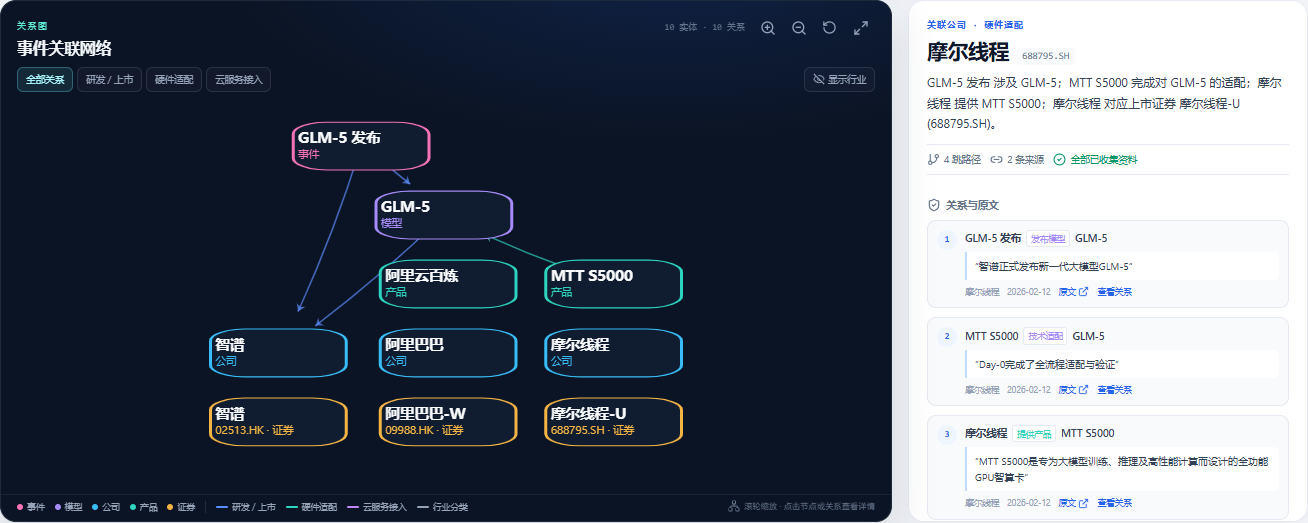
\includegraphics[width=\linewidth,height=5.7cm,keepaspectratio]{generated/new_overview.png}
\end{center}
\end{frame}

\begin{frame}{资料导入前后的查询结果}\relax
\Intro{初始图谱暂不包含 GLM-5 的适配事实，本页比较补入该事实前后的结果。}
\begin{columns}[T,onlytextwidth]
\column{.47\textwidth}
\Head{导入前：2 只证券}
智谱、阿里巴巴。
\Gap
\Head{导入后：3 只证券}
增加摩尔线程，路径经由 MTT S5000 的适配关系。
\column{.48\textwidth}
{\fontsize{11.7}{15}\selectfont
\begin{tabularx}{\linewidth}{@{}X r@{}}
\toprule
图谱记录 & 变化\\
\midrule
关联证券数 & 2 $\rightarrow$ 3\\
新增节点 & 1 个适配事件\\
新增关系 & 3 条\\
重复导入 & 0 个新增事实\\
\bottomrule
\end{tabularx}}
\end{columns}
\end{frame}

\begin{frame}{按资料公开日期查询}\relax
\Intro{以已收集的 DeepSeek-R1 资料为例，查看不同日期能够形成的证券路径。}
{\fontsize{11.7}{15}\selectfont
\begin{tabularx}{\linewidth}{@{}l X c@{}}
\toprule
查询截止日 & 截至该日新增的关联 & 累计证券数\\
\midrule
2025-01-20 & R1 发布；尚未形成完整证券路径 & 0\\
2025-02-03 & 腾讯云、百度千帆接入模型 & 2\\
2025-02-05 & 再加入海光 DCU 适配、中国电信云接入 & 4\\
\bottomrule
\end{tabularx}}
\Gap
\Head{日期处理}
逐条检查路径中的来源日期；任何一条关系晚于截止日，就不计入该证券。\par
未核实发布日期的资料只登记采集时间，不用于更早日期的查询。
\end{frame}

\begin{frame}{抽取初试：结果与主要问题}\relax
\Intro{在提供实体目录的条件下，对 6 段文本进行定向抽取，检查流程并定位问题。}
\begin{columns}[T,onlytextwidth]
\column{.43\textwidth}
{\fontsize{11.6}{15}\selectfont
\begin{tabularx}{\linewidth}{@{}X r@{}}
\toprule
核对项 & 结果\\
\midrule
正例目标关系 & 5 条\\
精确三元组匹配 & 4 条\\
共同提及负例 & 1 段\\
负例中生成的关系 & 0 条\\
\bottomrule
\end{tabularx}}
\column{.52\textwidth}
\Head{主要差异：研发主体的组织层级}
Qwen3 抽取主体为 \textbf{Alibaba Cloud}，与原文一致；参考标注采用\textbf{阿里巴巴集团}。
\Gap
研发关系类型一致，差异涉及主体层级。需复核参考标注与实体映射，并用独立标注集评估。
\end{columns}
\end{frame}

\begin{frame}{GLM-5 发布后的行情}\relax
{\fontsize{11.5}{15}\selectfont
5 日窗口内，智谱累计上涨 56.22\%，恒生指数下降 1.64\%。各序列以事件前一交易日收盘值归一为 100。}
\begin{center}
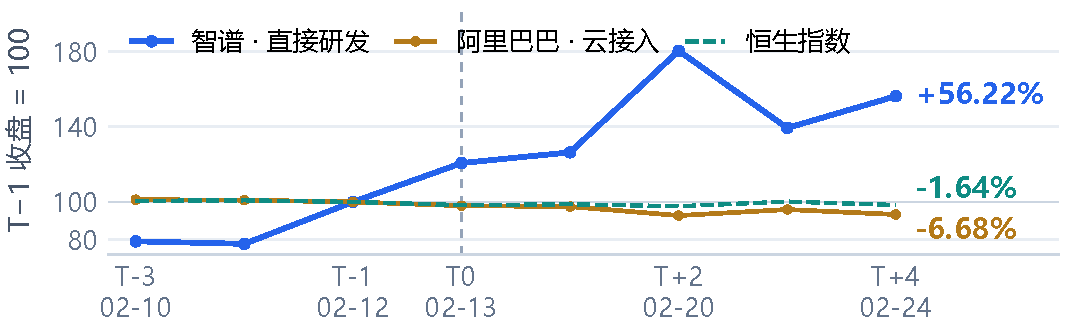
\includegraphics[width=13.3cm,height=4.5cm,keepaspectratio]{generated/market_roles.pdf}
\end{center}
\end{frame}

\section{后续计划}
\begin{frame}{后续工作}\relax
{\fontsize{11.8}{15.5}\selectfont
\begin{tabularx}{\linewidth}{@{}p{2.7cm} X p{4.4cm}@{}}
\toprule
方向 & 主要工作 & 验证方式\\
\midrule
组织与时间 & 补充集团关系，核实公告日期 & 复核公司与证券映射\\[2mm]
抽取评估 & 标注约 60 段文本，含共同提及负例 & 分类型统计 P/R/F1\\[2mm]
连续更新 & 按日期分三批导入，并重复输入 & 对照全量构建，检查重复事实\\
\bottomrule
\end{tabularx}}
\end{frame}

\appendix
\section*{}
\begin{frame}{关系类型与语义定义}\relax
\begin{tikzpicture}[remember picture,overlay]
\begin{scope}[shift={(current page.north west)},x=.23621875pt,y=-.236222222pt]
\node[anchor=north west,inner sep=0pt,outer sep=0pt,align=left,text=Navy,text width=410.07575pt,font={\fontsize{10.3}{13.081}\selectfont }] at (92,220) {拟新增组织归属关系，研发主体保留原文对应层级。};
\path[fill=FBlue!9,draw=Line,line width=.25pt] (92,285) rectangle (572,355);
\node[anchor=north west,inner sep=0pt,outer sep=0pt,align=left,text=Navy,text width=106.77088pt,font={\fontsize{10}{12.700}\selectfont\bfseries }] at (106,297) {关系类型};
\path[fill=FBlue!9,draw=Line,line width=.25pt] (572,285) rectangle (1272,355);
\node[anchor=north west,inner sep=0pt,outer sep=0pt,align=left,text=Navy,text width=158.73900pt,font={\fontsize{10}{12.700}\selectfont\bfseries }] at (586,297) {起点 $\rightarrow$ 终点};
\path[fill=FBlue!9,draw=Line,line width=.25pt] (1272,285) rectangle (1828,355);
\node[anchor=north west,inner sep=0pt,outer sep=0pt,align=left,text=Navy,text width=124.72350pt,font={\fontsize{10}{12.700}\selectfont\bfseries }] at (1286,297) {含义};
\path[fill=white,draw=Line,line width=.25pt] (92,355) rectangle (572,418);
\node[anchor=north west,inner sep=0pt,outer sep=0pt,align=left,text=Navy,text width=106.77088pt,font={\fontsize{9.5}{12.065}\selectfont }] at (106,367) {\texttt{DEVELOPED\_BY}};
\path[fill=white,draw=Line,line width=.25pt] (572,355) rectangle (1272,418);
\node[anchor=north west,inner sep=0pt,outer sep=0pt,align=left,text=Navy,text width=158.73900pt,font={\fontsize{9.5}{12.065}\selectfont }] at (586,367) {Model $\rightarrow$ Company / OrgUnit};
\path[fill=white,draw=Line,line width=.25pt] (1272,355) rectangle (1828,418);
\node[anchor=north west,inner sep=0pt,outer sep=0pt,align=left,text=Navy,text width=124.72350pt,font={\fontsize{9.5}{12.065}\selectfont }] at (1286,367) {模型的研发主体};
\path[fill=white,draw=Line,line width=.25pt] (92,418) rectangle (572,481);
\node[anchor=north west,inner sep=0pt,outer sep=0pt,align=left,text=Navy,text width=106.77088pt,font={\fontsize{9.5}{12.065}\selectfont }] at (106,430) {\texttt{PART\_OF}（拟新增）};
\path[fill=white,draw=Line,line width=.25pt] (572,418) rectangle (1272,481);
\node[anchor=north west,inner sep=0pt,outer sep=0pt,align=left,text=Navy,text width=158.73900pt,font={\fontsize{9.5}{12.065}\selectfont }] at (586,430) {OrgUnit $\rightarrow$ Company};
\path[fill=white,draw=Line,line width=.25pt] (1272,418) rectangle (1828,481);
\node[anchor=north west,inner sep=0pt,outer sep=0pt,align=left,text=Navy,text width=124.72350pt,font={\fontsize{9.5}{12.065}\selectfont }] at (1286,430) {经证据核验的组织归属};
\path[fill=white,draw=Line,line width=.25pt] (92,481) rectangle (572,544);
\node[anchor=north west,inner sep=0pt,outer sep=0pt,align=left,text=Navy,text width=106.77088pt,font={\fontsize{9.5}{12.065}\selectfont }] at (106,493) {\texttt{LISTED\_AS}};
\path[fill=white,draw=Line,line width=.25pt] (572,481) rectangle (1272,544);
\node[anchor=north west,inner sep=0pt,outer sep=0pt,align=left,text=Navy,text width=158.73900pt,font={\fontsize{9.5}{12.065}\selectfont }] at (586,493) {Company $\rightarrow$ Stock};
\path[fill=white,draw=Line,line width=.25pt] (1272,481) rectangle (1828,544);
\node[anchor=north west,inner sep=0pt,outer sep=0pt,align=left,text=Navy,text width=124.72350pt,font={\fontsize{9.5}{12.065}\selectfont }] at (1286,493) {公司对应的上市证券};
\path[fill=white,draw=Line,line width=.25pt] (92,544) rectangle (572,607);
\node[anchor=north west,inner sep=0pt,outer sep=0pt,align=left,text=Navy,text width=106.77088pt,font={\fontsize{9.5}{12.065}\selectfont }] at (106,556) {\texttt{PRODUCES}};
\path[fill=white,draw=Line,line width=.25pt] (572,544) rectangle (1272,607);
\node[anchor=north west,inner sep=0pt,outer sep=0pt,align=left,text=Navy,text width=158.73900pt,font={\fontsize{9.5}{12.065}\selectfont }] at (586,556) {Company $\rightarrow$ Product};
\path[fill=white,draw=Line,line width=.25pt] (1272,544) rectangle (1828,607);
\node[anchor=north west,inner sep=0pt,outer sep=0pt,align=left,text=Navy,text width=124.72350pt,font={\fontsize{9.5}{12.065}\selectfont }] at (1286,556) {公司提供的硬件或平台产品};
\path[fill=white,draw=Line,line width=.25pt] (92,607) rectangle (572,670);
\node[anchor=north west,inner sep=0pt,outer sep=0pt,align=left,text=Navy,text width=106.77088pt,font={\fontsize{9.5}{12.065}\selectfont }] at (106,619) {\texttt{SUPPORTS\_MODEL}};
\path[fill=white,draw=Line,line width=.25pt] (572,607) rectangle (1272,670);
\node[anchor=north west,inner sep=0pt,outer sep=0pt,align=left,text=Navy,text width=158.73900pt,font={\fontsize{9.5}{12.065}\selectfont }] at (586,619) {Product $\rightarrow$ Model};
\path[fill=white,draw=Line,line width=.25pt] (1272,607) rectangle (1828,670);
\node[anchor=north west,inner sep=0pt,outer sep=0pt,align=left,text=Navy,text width=124.72350pt,font={\fontsize{9.5}{12.065}\selectfont }] at (1286,619) {硬件技术适配};
\path[fill=white,draw=Line,line width=.25pt] (92,670) rectangle (572,733);
\node[anchor=north west,inner sep=0pt,outer sep=0pt,align=left,text=Navy,text width=106.77088pt,font={\fontsize{9.5}{12.065}\selectfont }] at (106,682) {\texttt{HOSTS\_MODEL}};
\path[fill=white,draw=Line,line width=.25pt] (572,670) rectangle (1272,733);
\node[anchor=north west,inner sep=0pt,outer sep=0pt,align=left,text=Navy,text width=158.73900pt,font={\fontsize{9.5}{12.065}\selectfont }] at (586,682) {Product $\rightarrow$ Model};
\path[fill=white,draw=Line,line width=.25pt] (1272,670) rectangle (1828,733);
\node[anchor=north west,inner sep=0pt,outer sep=0pt,align=left,text=Navy,text width=124.72350pt,font={\fontsize{9.5}{12.065}\selectfont }] at (1286,682) {云推理服务接入};
\path[fill=white,draw=Line,line width=.25pt] (92,733) rectangle (572,796);
\node[anchor=north west,inner sep=0pt,outer sep=0pt,align=left,text=Navy,text width=106.77088pt,font={\fontsize{9.5}{12.065}\selectfont }] at (106,745) {\texttt{RELEASED\_MODEL}};
\path[fill=white,draw=Line,line width=.25pt] (572,733) rectangle (1272,796);
\node[anchor=north west,inner sep=0pt,outer sep=0pt,align=left,text=Navy,text width=158.73900pt,font={\fontsize{9.5}{12.065}\selectfont }] at (586,745) {Event $\rightarrow$ Model};
\path[fill=white,draw=Line,line width=.25pt] (1272,733) rectangle (1828,796);
\node[anchor=north west,inner sep=0pt,outer sep=0pt,align=left,text=Navy,text width=124.72350pt,font={\fontsize{9.5}{12.065}\selectfont }] at (1286,745) {模型发布事件};
\path[fill=white,draw=Line,line width=.25pt] (92,796) rectangle (572,859);
\node[anchor=north west,inner sep=0pt,outer sep=0pt,align=left,text=Navy,text width=106.77088pt,font={\fontsize{9.5}{12.065}\selectfont }] at (106,808) {\texttt{CONCERNS}};
\path[fill=white,draw=Line,line width=.25pt] (572,796) rectangle (1272,859);
\node[anchor=north west,inner sep=0pt,outer sep=0pt,align=left,text=Navy,text width=158.73900pt,font={\fontsize{9.5}{12.065}\selectfont }] at (586,808) {Event $\rightarrow$ 相关实体};
\path[fill=white,draw=Line,line width=.25pt] (1272,796) rectangle (1828,859);
\node[anchor=north west,inner sep=0pt,outer sep=0pt,align=left,text=Navy,text width=124.72350pt,font={\fontsize{9.5}{12.065}\selectfont }] at (1286,808) {事件涉及的对象};
\path[fill=white,draw=Line,line width=.25pt] (92,859) rectangle (572,922);
\node[anchor=north west,inner sep=0pt,outer sep=0pt,align=left,text=Navy,text width=106.77088pt,font={\fontsize{9.5}{12.065}\selectfont }] at (106,871) {\texttt{BELONGS\_TO}};
\path[fill=white,draw=Line,line width=.25pt] (572,859) rectangle (1272,922);
\node[anchor=north west,inner sep=0pt,outer sep=0pt,align=left,text=Navy,text width=158.73900pt,font={\fontsize{9.5}{12.065}\selectfont }] at (586,871) {实体 $\rightarrow$ Industry};
\path[fill=white,draw=Line,line width=.25pt] (1272,859) rectangle (1828,922);
\node[anchor=north west,inner sep=0pt,outer sep=0pt,align=left,text=Navy,text width=124.72350pt,font={\fontsize{9.5}{12.065}\selectfont }] at (1286,871) {仅作行业分类，不推导证券};
\end{scope}
\end{tikzpicture}
\end{frame}

\begin{frame}{行情计算方法}\relax
\Intro{采用腾讯财经前复权日线，对照同日期的指数描述市场表现。}
\begin{columns}[T,onlytextwidth]
\column{.48\textwidth}
\Head{交易窗口}
披露时间只有日期时，采用之后首个交易日作为 T$_0$。基期为 T$_{-1}$ 收盘。
\Gap
1、3、5 日窗口分别截至 T$_0$、T$_{+2}$、T$_{+4}$；按各市场实际交易日顺延。
\Gap
GLM-5：T$_0$ 为 2026-02-13，5 日窗口截至 2026-02-24。
\column{.48\textwidth}
\Head{累计收益与基准}
\[
  R_k=\frac{P_{T_{k-1}}}{P_{T_{-1}}}-1
\]
基准使用同一组日期；相对基准值为累计收益的简单百分点差。
\Gap
港股以恒生指数、A 股以\mbox{科创50}为基准；未上市或行情不足时不计算收益。
\end{columns}
\end{frame}

\begin{frame}{主要数据来源}\relax
{\fontsize{11.3}{15}\selectfont
\begin{tabularx}{\linewidth}{@{}p{3.1cm} X p{2.7cm}@{}}
\toprule
来源 & 资料内容 & 公开日期\\
\midrule
DeepSeek 官方 & \href{https://api-docs.deepseek.com/news/news250120/}{DeepSeek-R1 发布} & 2025-01-20\\
阿里云官方 & \href{https://www.alibabacloud.com/en/press-room/alibaba-introduces-qwen3-setting-new-benchmark}{Qwen3 发布与模型信息} & 2025-04-29\\
Z.ai 官方 & \href{https://z.ai/blog/glm-5}{GLM-5 技术博文} & 2026-02-12\\
摩尔线程官方 & \href{https://www.mthreads.com/news/280}{MTT S5000 适配 GLM-5} & 2026-02-12\\
阿里云百炼文档 & GLM-5、MiniMax-M2.5 推理服务接入 & 未核实\\
交易所文件 & 公司名称、证券代码、上市日期 & 逐份记录\\
\bottomrule
\end{tabularx}}
\vfill
\Caption{完整登记见 data/sources.json：共 \SourceCount{} 条，包含发布方、原始链接、日期口径与短摘录。未知发布日期的动态文档另记采集时间。}
\end{frame}

\end{document}
